\documentclass[11pt]{article}
\usepackage[margin=1in]{geometry}
\usepackage{amsmath,amsthm,amssymb}
\usepackage{enumitem, graphicx, float, caption}
\usepackage{amsmath}
\usepackage{bm}
\usepackage{parskip}
\usepackage{lipsum}
\usepackage{tikz}
\usepackage{listings}
\usepackage{xcolor}
\usepackage{float}
\usepackage{subcaption}
\usepackage{graphicx}
\usepackage[utf8]{inputenc}
\usetikzlibrary{arrows.meta}

\definecolor{codegreen}{rgb}{0,0.6,0}
\definecolor{codegray}{rgb}{0.5,0.5,0.5}
\definecolor{codepurple}{rgb}{0.58,0,0.82}
\definecolor{backcolour}{rgb}{0.95,0.95,0.92}

\lstdefinestyle{mystyle}{
    backgroundcolor=\color{backcolour},
    commentstyle=\color{codegreen},
    keywordstyle=\color{magenta},
    numberstyle=\tiny\color{codegray},
    stringstyle=\color{codepurple},
    basicstyle=\ttfamily\scriptsize,
    breakatwhitespace=false,
    breaklines=true,
    captionpos=b,
    keepspaces=true,
    numbers=left,
    numbersep=5pt,
    showspaces=false,
    showstringspaces=false,
    showtabs=false,
    tabsize=2
}

\lstset{xleftmargin=.020\textwidth, xrightmargin=.020\textwidth}

\setcounter{MaxMatrixCols}{26}
\setlength\parindent{0pt}
\counterwithin{equation}{enumi}


\begin{document}
    \author{Nathan Burwig \\ MATH 87 Math Modeling} 
    \title{Midterm 2}
    \maketitle

    \section{Introduction}
    This is the midterm for Math Modelling (MATH 087) where we explore the
    aspects of the page rank system in a couple of smaller models, as well as
    some large examples.

    Google uses an algorithm called PageRank to rank web-pages by importance.
    The PageRank algorithm was originally formulated using a Markov Chain.
    Because of this, we can simulate it without a terrible amount of difficulty
    using our knoledge of Markov Chains.

    We know Markov chains can be represented by directed graphs with weight
    over edges connecting nodes. Thus we can write an adjacency matrix that
    shows which nodes are connected to which. We then assume that there is an
    equal probability of moving from one node, to any of the next nodes. So the
    weight over the edges from one node, to three nodes, will be $\frac{1}{3} $
    each.

    We know this is meant to represent a web experience, thus we know that at
    any point the user can stop clicking links (switching between nodes) so we
    can have a sink node where other nodes go to. From the sink node, we can
    consider that the user can then go to any other node in the graph with
    equal probability. Thus, if our adjacency matrix contains a sink (ie a
    column of zeros) then we can replace it with a column of ones.
    
    \section{The Problems}
    \begin{enumerate}
        \item  \textbf{A brief bit of math}

          Given an adjacently matrix $A$, complete the following
          description of the i,j entry of the corresponding PageRank
          transition matrix $C$ for the probability $p$.
          \begin{enumerate}
              \item If the j-th column of the matrix $A$ is equal to
                  \textbf{0}, then for each \lstinline{i = 0,...,n-1:} what is
                  $C_{i,j}$?

                  We know that $C = (1-p)T_1 + \frac{p}{n} \mathbf{J_n}$ for
                  $\mathbf{J_n}$ being an $n \times n$ matrix of ones. If the
                  j-th column of A is all zeros, then we can clearly see that
                  $T_1$ will have a column of ones, thus we should anticipate
                  our $C$ matrix to have values $\frac{1}{n} $ in $C_{i,j}$. 

              \item Suppose now the sum of the entires of the j-th column of
                  the matrix A is equal to $s > 0$, then...

                  If $A_{i,j} = 0$, then $C_{i,j} = \frac{p}{n}$

                  If $A_{i,j} = 1$, then $C_{i,j} = \frac{n-(L-n)}{Ln}$ 

                  We get this just from expanding out the expression for C and
                  generalizing.
          \end{enumerate}

      The above will be useful to us when going to write the code for the next
      problem.

      \item \textbf{Transition Matrices}

        For this problem, we wish to develop a python function to create a
        transition matrix from an adjacenty matrix. For this, we need to keep
        in mind the things we solved in part one. Namely how the matrices react
        to having columns of zeros or zeros in the A matrix.
        \begin{lstlisting}[style=mystyle, linewidth=0.94\linewidth,
                           language=Python, gobble=8, caption=make\_transition]
            ## make_transition is a function that takes in an adjacency matrix and
            ## produces a transition matrix under a given sets of rules and using a
            ## probability damping factor in accordance with the pagerank system
            def make_transition(A, p):
                (n, m) = A.shape
                big_c = np.zeros((n,n))
            
                # check if square
                if n == m:
                    # get number of ones in a column
                    for i in range(n):
                        col = A[:, i]
                        c = 0
            
                        #count number of ones in a column
                        for j in range(n):
                            if col[j] == 1:
                                c = c + 1
            
                        # a fix for if the column is of zeros, replaces with one
                        if c == 0:
                            col = np.ones(n)
                            c = n
            
                        # populate the big_C matrix with the correct values given
                        # part 1
                        for k in range(n):
                            if col[k] == 1:
                                big_c[k][i] = (n + (c - n) * p)/(c * n)
                            else:
                                big_c[k][i] = p/n
                                
                # return the final array
                return big_c
        \end{lstlisting} 

        We can test this against any number of matrices, but testing against
        the test sample given in the assignment. Doing so gives the following
        output...
        \begin{lstlisting}[style=mystyle, linewidth=0.92\linewidth,
                           language=Python, gobble=8, caption=testing
                           make\_transition]
            print("Transition Matrix:")
            print(P, "\n")
            
            print("Adjacency Matrix:")
            print(make_transition(P, .8))
        \end{lstlisting}
        \newpage
        \begin{verbatim}[output]
            Transition Matrix:
            [[0 0 0 0 1]
             [1 0 0 0 1]
             [1 1 0 0 1]
             [1 0 1 0 1]
             [0 1 0 1 1]] 
            
            Adjacency Matrix:
            [[0.16000 0.16000 0.16000 0.16000 0.20000]
             [0.22667 0.16000 0.16000 0.16000 0.20000]
             [0.22667 0.26000 0.16000 0.16000 0.20000]
             [0.22667 0.16000 0.36000 0.16000 0.20000]
             [0.16000 0.26000 0.16000 0.36000 0.20000]]
        \end{verbatim}
        So we can clearly see that it is operating as expected given the
        output. This is good. We can now take any adjacency matrix and convert
        it into a transition matrix.
        
    \item \textbf{Eigenvector Analysis}

        We now want to apply some of these tools and ideas that we've built
        up here. We know we can make a transition matrix out of an adjacency
        matrix in a way that has an associated dampening factor such that we
        have an approximate PageRank setup.

        We can do this setup for the following di-graph.

        \begin{center}
            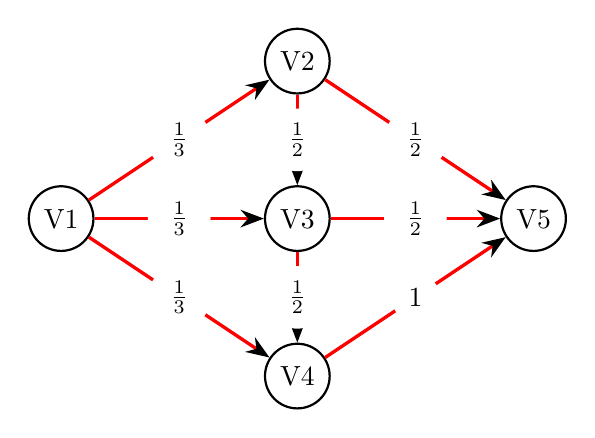
\begin{tikzpicture}
                \begin{scope}[every node/.style = {circle, thick, draw}]
                    \node (V1) at (0, 0)    {V1};
                    \node (V2) at (3, 2)    {V2};
                    \node (V3) at (3, 0)    {V3};
                    \node (V4) at (3, -2)   {V4};
                    \node (V5) at (6, 0)    {V5};
                \end{scope}        

                \begin{scope}[>={Stealth[black]},
                                every node/.style={fill=white,circle},
                                every edge/.style={draw=red,very thick}]
                     \path [->] (V1) edge node {$\frac{1}{3}$} (V2);
                     \path [->] (V1) edge node {$\frac{1}{3}$} (V3);
                     \path [->] (V1) edge node {$\frac{1}{3}$} (V4);
                     \path [->] (V2) edge node {$\frac{1}{2}$} (V3);
                     \path [->] (V3) edge node {$\frac{1}{2}$} (V4);
                     \path [->] (V2) edge node {$\frac{1}{2}$} (V5);
                     \path [->] (V3) edge node {$\frac{1}{2}$} (V5);
                     \path [->] (V4) edge node {1} (V5);
                \end{scope}
            \end{tikzpicture}
        \end{center}
        This has the same adjacency matrix as the example used above in the
        code. I have marked the probabilities associated with each edge here,
        and it is worth noting that this is not the graph representing the
        transition matrix with the column of ones included to account for the
        sink node. That would be represented by node five connecting to every
        node in the graph with a weight of $\frac{1}{5}$

        We now wish to determine the 1-eigenvector of the system. This vector,
        normalized such that it is a probability vector, will give us the
        long-term probability that a given user will be on a given site. We can
        utilize the \texttt{numpy.linalg.eig()} function to determine the
        eigenvalues of our given matrix. From there, we can normalize the
        vector, and this will be a probability vector which we can then
        interpret.
        \newpage

        \begin{center}
            \begin{lstlisting}[style=mystyle, linewidth=0.94\linewidth, 
                                language=Python, gobble=9, caption=Finding
                                eigenvals and eigenvectors]
                ## b is associated with p=0.8 and c with p=0.4
                e_val_b, e_vec_b = np.linalg.eig(b)
                e_val_c, e_vec_c = np.linalg.eig(c) 

                ## determine which eigenvalue is of value one
                print("eigen val for first entry in e_val_b:  ", e_val_b[0])
                print("eigen val for first entry in e_val_c:  ", e_val_c[0], "\n")

                ## name the vector of interest as the one eigenvector
                ovb = e_vec_b[:,0]
                print(ovb)
                ovc = e_vec_c[:,0]
                print(ovc)
            \end{lstlisting}
        \end{center}
        We associate \texttt{ovb} with the eigenvector of the \texttt{p=.8} and
        \texttt{ovc} with \texttt{p=.4}. The output of this is then...
        \begin{lstlisting}[basicstyle=\ttfamily\footnotesize]
        [output]
            eigen val for first entry in e_val_b:   (1+0j)
            eigen val for first entry in e_val_c:   (1.0000000000000004+0j)

            ovb:   [-0.3759169 +0.j -0.40097802+0.j -0.44107583+0.j 
                    -0.48919319+0.j -0.51385334+0.j]
            ovc:   [0.24682597+0.j 0.29619116+0.j 0.38504851+0.j 
                    0.52722026+0.j 0.65201547+0.j]
        \end{lstlisting}
        We can normalize these eigenvectors to get the following. I wrote a
        small piece of code that outputs information of interest relating to
        the normalized vectors, so i'll just print the output from that.

        \begin{minipage}[t]{0.48\linewidth}
            \begin{lstlisting}[basicstyle=\ttfamily\footnotesize, gobble=8]
            [output p=.8]
                NORMALISED VECTOR:
                [0.16925438-0.j 
                 0.180538  -0.j 
                 0.1985918 -0.j 
                 0.22025636-0.j 
                 0.23135945-0.j] 

                NORMALISATION TEST:
                (1+0j)
                
                FORMATTED VECTOR:
                (0.1692543780465788-0j)
                (0.18053800324968394-0j)
                (0.19859180357465242-0j)
                (0.22025636396461457-0j)
                (0.23135945116447024-0j)
            \end{lstlisting}
        \end{minipage} \hfill \vline \hfill%
        \begin{minipage}[t]{0.48\linewidth}
            \begin{lstlisting}[basicstyle=\ttfamily\footnotesize, gobble=8]
            [output p=.4]
                NORMALISED VECTOR:
                [0.11712894+0.j 
                 0.14055472+0.j 
                 0.18272114+0.j 
                 0.25018741+0.j
                 0.3094078 +0.j] 

                NORMALISATION TEST:
                (1+0j)
                
                FORMATTED VECTOR:
                (0.11712893553223379+0j)
                (0.14055472263868063+0j)
                (0.1827211394302849+0j)
                (0.25018740629685166+0j)
                (0.309407796101949+0j)
            \end{lstlisting}
        \end{minipage}

        We can do a power iteration of our adjacency matrix to see if the
        values line up, and we see, when running the power iteration 200
        times...

        \begin{lstlisting}[style=mystyle, linewidth=0.94\linewidth, 
                            language=Python, gobble=9, caption=Power iteration]
                aa = (np.linalg.matrix_power(a,200))
                cc = (np.linalg.matrix_power(c,200))
                print("**aa:\n", aa[:,0])
                print("**cc:\n", cc[:,0])
        \end{lstlisting}
        \begin{lstlisting}[basicstyle=\ttfamily\footnotesize]
        [output]
            **aa:
            [0.16925 0.18054 0.19859 0.22026 0.23136]
            **cc:
            [0.11713 0.14055 0.18272 0.25019 0.30941]
        \end{lstlisting}

        So we can see that in the end we recover the same eigenvectors
        regardless of power iteration or more typical eigenvector analysis.
        This is good! It means our matrix is stochastic and following all the
        rules we exepect.
        \medskip

    \item \textbf{A New Graph}

        We now look at the following diagram...

        \begin{center}
            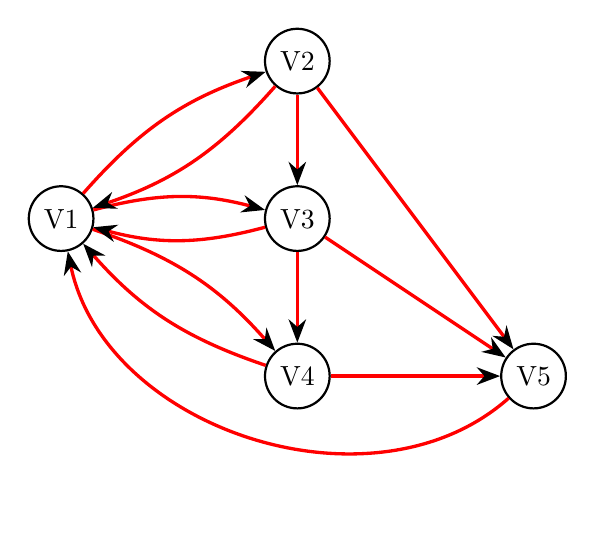
\begin{tikzpicture}
                \begin{scope}[every node/.style = {circle, thick, draw}]
                    \node (V1) at (0, 0)    {V1};
                    \node (V2) at (3, 2)    {V2};
                    \node (V3) at (3, 0)    {V3};
                    \node (V4) at (3, -2)   {V4};
                    \node (V5) at (6, -2)    {V5};
                \end{scope}        

                \begin{scope}[>={Stealth[black]},
                                every node/.style={fill=white,circle},
                                every edge/.style={draw=red,very thick}]
                     \path [->] (V1) edge[bend left=15] (V2);
                     \path [->] (V1) edge[bend left=15] (V3);
                     \path [->] (V1) edge[bend left=15] (V4);
                     
                     \path [->] (V2) edge (V5);
                     \path [->] (V2) edge (V3);
                     \path [->] (V2)[bend left=15] edge (V1);

                     \path [->] (V3) edge (V4);
                     \path [->] (V3) edge (V5);
                     \path [->] (V3) edge[bend left=15] (V1);

                     \path [->] (V4) edge (V5);
                     \path [->] (V4) edge[bend left=15] (V1);

                     \path [->] (V5) edge[bend left=60] (V1);
                \end{scope}
            \end{tikzpicture}
        \end{center}

        We can create an adjacency matrix for this diagram that looks as
        follows (note, I've indexed the nodes such that index zero is node one
        and so on for each row and column, in the same way that the initial
        matrix was created.)
        \[
            A = 
            \begin{bmatrix}
                0   &   1   &   1   &   1   &   1   \\
                1   &   0   &   0   &   0   &   0   \\
                1   &   1   &   0   &   0   &   0   \\
                1   &   0   &   1   &   0   &   0   \\
                0   &   1   &   0   &   1   &   0
            \end{bmatrix}
        \]
        We can run the same set analyses on this as we ran on the previous
        parts. I'll save us the hassle of writing out all the same code again
        and skip to the conclusions...

        \begin{minipage}[t]{0.48\linewidth}
            \begin{lstlisting}[basicstyle=\ttfamily\footnotesize, gobble=8]
            [output p=.8]
                NORMALISED VECTOR:
                [0.24840514+0.j 
                 0.17656034+0.j 
                 0.18833103+0.j 
                 0.19539345+0.j
                 0.19131003+0.j]

                NORMALISATION TEST:
                (0.9999999999999999+0j)
                
                FORMATTED VECTOR:
                (0.248405144227276+0j)
                (0.17656034294848497+0j)
                (0.18833103247838412+0j)
                (0.1953934461963234+0j)
                (0.19131003414953138+0j)
            \end{lstlisting}
        \end{minipage} \hfill \vline \hfill%
        \begin{minipage}[t]{0.48\linewidth}
            \begin{lstlisting}[basicstyle=\ttfamily\footnotesize, gobble=8]
            [output p=.4]
                NORMALISED VECTOR:
                [0.31989529-0.j 
                 0.14397906-0.j 
                 0.17277487-0.j 
                 0.19581152-0.j
                 0.16753927-0.j] 

                NORMALISATION TEST:
                (1+0j)
                
                FORMATTED VECTOR:
                (0.31989528795811517-0j)
                (0.14397905759162308-0j)
                (0.17277486910994766-0j)
                (0.1958115183246073-0j)
                (0.16753926701570687-0j)
            \end{lstlisting}
        \end{minipage}

        We can note a distinct difference bewtween the analysis in question 2,
        vs this question. The most notable feature is that the higher values of
        the eigenvectors are not associated with the lower numbered nodes
        (nodes 1, 2, and 3) whereas in the previous example we see the higher
        probabilities are associated with the higher numbered nodes (nodes 3,
        4, and 5). 

        Just by looking at the graph, this makes sense. We can see the graph is
        significantly more connected in this case around nodes 1-4, with the
        ability to go back and forth between 1 and 2, 3, and 4 as many times as
        you wish. Before, we could not do that, so it makes sense that on
        average you wouldn't expect to be on the lower numbered nodes as
        frequently. Now, however, there are more links to these nodes, so we
        would expect that in the long term, we have a higher probability of
        being on these nodes.
        \medskip


    \item  \textbf{The Perron-Frobenius Theorem}

        For any directed graph, explain whey the corresponding
        \texttt{PageRank} transition matrix of $\texttt{p > 0}$ is a stochastic
        matrix corresponding to a strongly connected aperiodic transition
        diagram. In particular, explain why the conclusion of the
        \textit{Perron-Frobenius Theorem} holds for this matrix.

        We start with an explanation of why the \texttt{PageRank} Transition
        matrix is \textit{stochastic}.

        We know the transition matrix must be stochastic, as the damping factor
        ensures that the sum of each of the columns of the transition matrix is
        exactly 1 by dividing by the total number of nodes. This is the
        definition of a stochastic matrix, and thus we know the transition
        matrix is stochastic.

        We know the transition matrix is \textit{strongly connected} as the
        damping factor is the probability that you stop and move to a random
        website in the group. Thus, at any point in the graph there is some
        chance that you will move to any other node in the graph, and
        because $p > 0$, we know that every node is connected with some
        probability $p$, thus the chain \textit{must} be strongly connected.

        Further, we know that there is some chance of moving between any nodes,
        including (possibly) the node you are currently on, there must be self
        cycles of length 1 at every node. Thus the graph is \textit{aperiodic}.

        Given that the graph is aperiodic and strongly connected, we know the
        Perron-Frobenius Theorem must hold, and that there is a single largest
        eigenvalue no greater than 1, and that all other eigenvalues have an
        absolute value between 1 and 0. This is exactly what we see in our
        \texttt{PageRank} simulations here, so this all makes sense.

    \item \textbf{A somewhat larger example}

        We now turn our heads to a different example. We have been given code
        to process a large \texttt{.json} file which contains information
        simulating the searchs for some animals as webpages, and we can use the
        \texttt{PageRanks} setup we have developed thus far, to run an analysis
        on this, and determine which nodes are most likely to be visited over
        time. 

        Using the code given in the assignment, we can initialize the adjacancy
        matrix from the \texttt{.json} file. After that, we can feed the array
        into our \texttt{make\_transition} function, to get the transition
        matrix, and then do the usual eigen vector method to get the long term
        probabilities for each website.

        The code to do all of this is given in the following.

        \begin{lstlisting}[style=mystyle, linewidth=0.94\linewidth, 
                            language=Python, gobble=8, caption=The analysis]
            ## The code to initialize the matrix A
            (ll, A) = adj_from_json("data.json")

            ## make the transition matrix and get it's eigen values
            A_a = make_transition(A, 0.8)
            e_vlA, e_vcA = np.linalg.eig(A_a)

            ## get the 1-eigenvector and normalize it, then print info
            ## using a previously created function
            eA = e_vcA[:,0]
            e_nA = normalize(eA)
            norm_inf(e_nA)
        \end{lstlisting}

        After doing this, it becomes clear that the eigenvector has been
        normalized. I will be putting some of the output below, but it takes up
        a rather large amount of space so I will be cutting out some of the
        middling values in order to save space.

        \begin{minipage}[t]{.48\linewidth}            
            \begin{center}
                \begin{lstlisting}[basicstyle=\ttfamily\footnotesize, gobble=10]
                [output p=.8]
                    NORMALISED VECTOR:
                    [0.01353617-0.j 
                     0.01061748-0.j 
                     0.01035092-0.j 
                        . . .
                     0.01049602-0.j 
                     0.01059754-0.j
                     0.01032602-0.j]

                    NORMALISATION TEST:
                    (1+0j)

                        . . .
                \end{lstlisting}
            \end{center}
        \end{minipage}\hfill \vline \hfill%
        \begin{minipage}[t]{.48\linewidth}
             So now we have our normalized eigenvector. We now need a way to
             figure out the top ten values in it, and which values are
             associated in the \texttt{ll} matrix. In order to do this, we can
             write a quick funciton that finds the top ten max values, by
             creating a copy of the array, then finding the max value within
             that copy, and storing it in a new list. Then, we can set that
             value to 0, such that we never find the same max twice. We can do
             this 10 times in a for loop, and then we will have our list of top
             ten websites ranked by \texttt{PageRank}.
        \end{minipage}
        \newpage

        The function we outlined above, looks as follows.

        \begin{lstlisting}[style=mystyle, linewidth=0.94\linewidth, 
                            language=Python, gobble=8, caption=Finding the top ten]
            def top_ten(e_nA):
                ## copy array to temp array so we don't change values in eigenvector
                temp = []
                for i in range(len(e_nA)):
                    temp.append(e_nA[i])

                ## array of max values
                maxes = []

                ## loop through 10 times finding max val in array, and copying
                for i in range(10):

                    ## find max val and index of max val
                    max = np.amax(temp)
                    ind = np.where(temp == max)[0]

                    ## find the associated animal in ll
                    animal = ll[int(ind)]

                    ## set index to zero so it doesn't find the same max twice
                    temp[int(ind)] = 0
                    
                    ## put the animal in the aray maxes
                    maxes.append(animal)
                    
                print(maxes)
        \end{lstlisting}

        Calling this on our $A$ array yields the following...

        \begin{lstlisting}[basicstyle=\ttfamily\footnotesize, gobble=8]
            ['Blue Whale', 'Ant', 'Donkey', 'Squirrel', 'Rook', 'Grouse', 
             'Fowl', 'Gerbil', 'Carp', 'Albatross']
        \end{lstlisting}

        Thus we have our top ten list.

        When we reduce the value of $p$ we find that we get the \textit{mostly}
        the same animals in the top ten, just in a different ordering. The
        reason, I suspect, for this has to do with the actual number of edges.
        If there are many more edges leading to the animals we found in our top
        ten, then we would expect that, regardless of our damping factor, you
        will still have a higher chance of being on those websites. The damping
        factor would just mean that you have a higher chance of randomly moving
        to one of any sites more frequently, so the lower you go, the less
        probably it is for that to happen. 

    \item \textbf{Citation Station}

        Does this system work the same way for something like paper citations
        where the edges are citations and the nodes papers containing those
        citations?

        I think this would work almost exactly the same. You could still have
        your damping factor enfore the Perron-Frobenious Theorem, and thus you
        still have a workable stochastic matrix. The setup is almost identical
        as you have your citations working as links. The $p$ factor would just
        be the chance that at any given point the user stops sifting through
        papers and decided to move to some random paper in the stack. 

        One thing worth noting, though, is that, while I think this proposal
        would work in theory, I don't know if it is exactly the best setup. If
        you go looking for papers on google, I feel like this would be
        appropriate, but the 1-eigenvector associated with this setup would be
        ranking the long term average probability of a paper being read, and
        not necessarily sort via merit or peer review. Just because a paper has
        plenty of citations, doesn't necessarily make it accurate, and thus I
        don't know if this system would be the best for sorting things by
        academic merit. However, it could work just fine in the sense that one
        could certainly setup a system that looks like this.
    \end{enumerate}
    

\end{document}
